% A simple template for LaTeX documents
% 
% To produce pdf run:
%   $ pdflatex paper.tex 
%


\documentclass[12pt]{article}

% Begin paragraphs with new line
\usepackage{parskip}  

% Change margin size
\usepackage[margin=1in]{geometry}   

% Graphics Example:  (PDF's make for good plots)
\usepackage{graphicx}               
% \centerline{\includegraphics{figure.pdf}}

% subfigures, side by side
\usepackage{subcaption}

% hyperlinks
\usepackage{hyperref}

% Blocks of code
\usepackage{listings}
\lstset{basicstyle=\ttfamily, title=\lstname}
% Insert code like this. replace `plot.R` with file name.
% \lstinputlisting{plot.R}

% Monospaced fonts
%\usepackage{inconsolata}
% GNU \texttt{make} is a nice tool.

% Supports proof environment
\usepackage{amsthm}

% Allows writing \implies and align*
\usepackage{amsmath}

% Allows mathbb{R}
\usepackage{amsfonts}

% Numbers in scientific notation
% \usepackage{siunitx}

% Use tables generated by pandas
\usepackage{booktabs}

% Allows umlaut and non ascii characters
\usepackage[utf8]{inputenc}

% Insert blank pages
\usepackage{afterpage}
%\afterpage{\null\newpage}

% norm and infinity norm
\newcommand{\norm}[1]{\left\lVert#1\right\rVert}
\newcommand{\inorm}[1]{\left\lVert#1\right\rVert_\infty}

% Statistics essentials
\newcommand{\iid}{\text{ iid }}
\newcommand{\Exp}{\operatorname{E}}
\newcommand{\Var}{\operatorname{Var}}
\newcommand{\Cov}{\operatorname{Cov}}


%%%%%%%%%%%%%%%%%%%%%%%%%%%%%%%%%%%%%%%%%%%%%%%%%%%%%%%%%%%%

\begin{document}

\title{Parallel Computing Through Code Analysis}
\date{\today}
\author{Clark Fitzgerald}
\maketitle

\begin{abstract}

%This is a proposal for the Statistics PhD Qualifying Exam in June 2017.

    Conventional systems for parallel programming require users to modify
    existing code to take full advantage of a platform's computational
    capabilities. In this proposal we consider automated code analysis
    methods to detect the potential for parallel execution in R code. The results of
    the analysis can then be used to programmatically rewrite and execute
    semantically equivalent parallel instructions, without requiring the
    user to modify their original code.  We consider a motivating case
    study analyzing the operating characteristics of California's highway
    traffic sensor stations on hundreds of gigabytes of traffic sensor
    data.

\end{abstract}

\section{Code, Data, Platform}
%%%%%%%%%%%%%%%%%%%%%%%%%%%%%%%%%%%%%%%%%%%%%%%%%%%%%%%%%%%%

\begin{figure}
\centering
\includegraphics[width=.5\linewidth]{workflow}
\caption{Given sequential code and a description of the data we seek
    a modified computational parallel plan tailored to a specific platform.}
\label{fig:workflow}
\end{figure}

For our purposes in this document, \textbf{code} is a script to be
executed.  \textbf{Data} could be data in memory, single or multiple files,
a memory-mapped file, a database, a parallel file system, etc.
\textbf{Platform} is the computing setup, such as a laptop with 4 cores, a
cluster of machines communicating over a network, or a server with 2 GPUs
and a high bandwidth connection. Knowing the combination of \{Code, Data,
Platform\} allows one to select an appropriate strategy for efficient
computation.  Figure \ref{fig:workflow} illustrates the high level goal of
modifying the code to run efficiently with a particular platform and data,
while preserving the semantics of the input code.

This project is in the spirit of compiling R, since it treats R code as a
set of high level directions, and generates alternative code for execution
\cite{lang2014enhancing}. In the future we hope to connect and extend this
project using recent work on compilation. Note that the system does not
invent new algorithms on the fly. However, it should be capable of tuning
existing parameters to the problem at hand.\footnote{An example of a
parameter to be tuned is the chunk size $n_j$ as described in
\ref{sec:sequential}.} 

\section{Motivating Example}
%%%%%%%%%%%%%%%%%%%%%%%%%%%%%%%%%%%%%%%%%%%%%%%%%%%%%%%%%%%%
\label{sec:pems}

The example in this section is interesting for the following reasons:
\begin{itemize}
    \item The results are relevant to domain scientists in traffic engineering.
    \item The size of the data exceeds the memory of a single server.
    \item Parallel programming can increase the speed by 1-2 orders of
        magnitude.
\end{itemize}

The California Department of Transportation (CalTrans) collects traffic data through
sensors embedded in highways. The sensors measure three quantities: count
of passing vehicles (flow), time during which a vehicle is directly above the
sensor (occupancy), and average velocity \cite{jia2001pems}.  Every thirty
seconds they produce a new data point. $43,680$ sensors in California
measuring 3 parameters multiplied by $2 \times 60 \times 24$ measurements
per day results in 377 million new data points per day.  CalTrans provides
the raw data for public download. It's organized into files containing
observations for one day for each of the 12 management districts in
California.

\begin{figure}
\centering
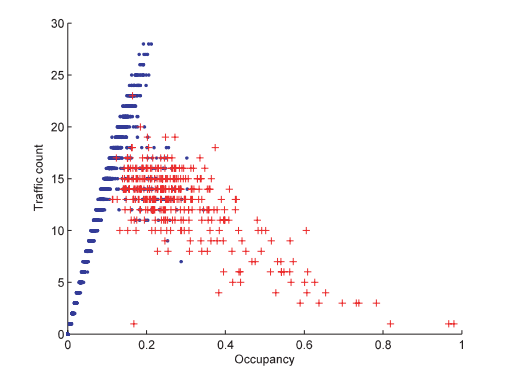
\includegraphics[width=.7\linewidth]{seminar/fundamental_diagram}
\caption{The fundamental diagram in traffic engineering.}
\label{fig:fundamental_diagram}
\end{figure}

Traffic engineers model traffic flow as a function of occupancy for each
sensor as in figure \ref{fig:fundamental_diagram}. This relationship is
called the \emph{fundamental diagram} because it captures the operating
characteristic of this section of road \cite{daganzo1997fundamentals}. 
Robust regression can be used to fit the fundamental diagram for one
station, approximating the minimization of the L1 norm of the residuals as
in \cite{li2011fundamental}.  From the R language this can be done easily
and efficiently, for example with the \texttt{rlm} (robust linear model)
function in the MASS package \cite{venables2013modern}. \texttt{rlm} can be
used as a building block for a user defined \texttt{fit\_fd} function, and
the fundamental diagram can be fit on a single station with
\texttt{fit\_fd(station1)}. Then all stations can be fitted
by grouping the data by station and
applying \texttt{fit\_fd()} to each group.
R code expresses this computation succintly:
%Allowing user defined functions keeps this flexible, facilitating research
%and experimentation. 

\begin{verbatim}
by(alldata, INDICES = station, FUN = fit_fd)
\end{verbatim}

I would like to apply this code to a subset of the data consisting of
observations in the San Francisco Bay Area for part of 2016.  This data is
134 GB on disk. It won't fit into memory, so this code won't run.  Even
if it did fit in memory, it would be slow because \texttt{by()} won't run
\texttt{fit\_fd()} in parallel across the 1000's of different
stations\footnote{ Depending on overhead it may be less efficient to run
\texttt{fit\_fd()} in parallel.}.

It would be easier to perform this computation if the data were
organized in files for each station rather than in files for each day.  One
approach is to reorganize the data on disk into this file structure. I
did this using a simple single threaded R program, and it took 23 hours to
run on the 2016 Bay Area data.  Throughput for a conventional hard disk is around
100 MB/s\footnote{Other technologies such as parallel filesystems can
increase throughput.}, so an approximate lower bound for reading then
writing this reorganized data is $2 * 134000 / 100$ seconds, or 45 minutes
for 134 GB.  The simple code is 30 times slower than this. Small
inefficiencies add up.

Another drawback is that the programmer must write very specific
instructions to reorganize the data for computations grouped by station.
Any parallel programming will make this even more specific to the data and
platform. Subsequent slight modifications of the analysis may warrant a
completely different approach. For example, using least squares instead of
robust regression allows the use of an updating algorithm such as provided
by the \texttt{biglm} package \cite{R-biglm}, so there is no need to have
all the data for one group in memory at once.

What if we had a system that could inspect the idiomatic R code above that
works on small data sets, and then automatically take steps to scale and to
parallelize the operations? It should also be capable of tuning for the
specifics of the platform and the data. This is the goal of the research.

\section{Simple Example}
%%%%%%%%%%%%%%%%%%%%%%%%%%%%%%%%%%%%%%%%%%%%%%%%%%%%%%%%%%%%

% Duncan:
% Come up with concrete and realistic examples.  Show how you would do things
% differently for different computational platform Go through this explicitly
% by hand to show the "ideal" transformed code (keep high level) Identify how
% you might identify these programmatically and what are some of the
% challenges

We use an intentionally simple example to see exactly what translated code might look
like.  Consider computing the mean,

\begin{equation}
    \bar{x} = \frac{1}{n} \sum_{i = 1}^n x_i
\label{eq:mean}
\end{equation}

where the $x_i$'s are
i.i.d. $\sim t(d)$.  In R this code is written:

\begin{verbatim}
xbar = mean(rt(n, d))
\end{verbatim}

Ordinarily, to evaluate this R will first build an intermediate vector $x =
(x_1, \dots, x_n)$ and then compute the mean. Eventually that unreferenced
intermediate vector will be garbage collected.\footnote{Reducing the use of
unnessary intermediate vectors would be helpful, but it's a second order
consideration.} Execution time increases linearly with $n$. Once $n$
becomes large enough this vector will no longer fit into available physical
memory, so the operating system will use swap space. On a machine with 8 GB
memory this happens when $O(n) = 10^9$, causing the execution time to
increase by an order of magnitude, roughly from 1 minute to 15 minutes.
Once $n$ exceeds memory and swap space R will not be able to allocate a
large enough object, and the computation will fail with a memory error.

\subsection{Sequential Execution}
\label{sec:sequential}

The following example illustrates how single threaded R can be modified to
work with a data set that does not fit into memory. I do this 
by breaking the computation into chunks. The code below not run in parallel,
but it does use the same functional programming patterns as parallel code. 

Suppose $n = p n_j$ for integers $p, n_j$.  The mean can be
expressed as 

\begin{equation}
    \bar{x} = \frac{1}{n} \sum_{j = 1}^p \sum_{i = 1}^{n_j} x_{ij}
    = \sum_{j = 1}^p \frac{n_j}{n} \bar{x}_j
\label{eq:mean_partial}
\end{equation}

Conceptually, $p$ is the number of chunks and $n_j$ is the size of each
chunk. Equation \ref{eq:mean_partial} can be directly translated into R
code as follows:

\begin{verbatim}
partial_means = replicate(p, mean(rt(n_j, d)))
xbar = mean(partial_means)
\end{verbatim}

In this code \texttt{replicate()} evaluates the expression
\texttt{mean(rt(n\_j, d))} $p$ times sequentially, storing the intermediate
results.  If $M$ is the size of physical memory in bytes then this code is
high performance in the sense that execution time will continue to be
linear while $n < O(M^2)$, just as it was for small $n < O(M)$. The memory
footprint is bounded since the intermediate vectors will be of length
$n_j$. So small chunk sizes use less memory. On the other hand, large chunk
sizes improve speed when computing on vectors in R, since the overhead of
the R interpreter is amortized. 

% In practice, vectors with at least
% 1000 elements are found to be large enough \cite{chambers2016extending}.
% I think it's here, but can't find it.

% TODO: Need more on the above?

\subsection{SNOW Cluster}

A common way to write parallel R code is through the SNOW package, which
stands for Simple Network Of Workstations.  Clusters created by SNOW
consist of independent worker R processes created by a manager process. The
processes communicate over network sockets, and they may be on one or many
physical machines.  This is the type of cluster used by partools to
implement Software Alchemy \cite{R-partools} \cite{matloff2014software}.
The following code implements equation \ref{eq:mean_partial} in SNOW:

\begin{verbatim}
library(parallel)
p = floor(detectCores(logical = FALSE) / 2)
n_j = n / p
cluster = makeCluster(p)
clusterExport(cluster, c("n_j", "d"))
partial_means = unlist(
    clusterEvalQ(cluster, mean(rt(n_j, d))))
xbar = mean(partial_means)
\end{verbatim}

Here's what each line of code does:

\begin{enumerate}
    \item \texttt{library(parallel)} loads the parallel package, which R
        includes as a recommended package.
    \item \texttt{p = floor(detectCores(logical = FALSE) / 2)}
        chooses the number of chunks in a principled way, to use half of
        the physical processors available on the platform. This respects
        other programs and users who may be on the system.
    \item \texttt{n\_j = n / p} chooses the chunk size based on $n$ and
        $p$. 
    \item \texttt{cluster = makeCluster(p)} makes a local cluster with $p$
        workers. Given an existing cluster I would skip this step.
    \item \texttt{clusterExport(cluster, c("n\_j", "d"))} sends the
        variables $n_j, d$ to the workers, so they will be available for
        the local computations.
        Using a system fork to create the cluster allows me to
        skip this step, since forked processes have access to the variables
        that existed when they were created.
    \item \texttt{clusterEvalQ(cluster, mean(rt(n\_j, d)))} sends the code
        \texttt{mean(rt(n\_j, d))} from the manager to be evaluated on each
        worker.
    \item \texttt{partial\_means = unlist(...)} converts the list data
        structure to the intermediate numeric vector.
    \item \texttt{xbar = mean(partial\_means)} finally computes the mean
        from the intermediate result.
\end{enumerate}

Given an existing cluster, this strategy is efficient, provided that the
network latency is much less than the time required to evaluate the code.
The manager sends only two numbers and the code \texttt{mean(rt(n\_j, d))}
for evaluation. The workers each return a single number. Therefore the
program avoids large data transfers.

% This parallel model is useful in
% statistics for independent simulations, cross validation, bootstrap, data
% chunking

\section{Code Analysis}
%%%%%%%%%%%%%%%%%%%%%%%%%%%%%%%%%%%%%%%%%%%%%%%%%%%%%%%%%%%%

Code analysis involves the following steps:

\begin{itemize}
    \item Parse the code, gathering dependency information as explained in
        section \ref{sec:expression_dependency}.

%    \item Fuse loops, combining vectorized operations where possible. For
%        example, if the temporary variable \texttt{tmp} isn't used later
%        then this code:
%\begin{verbatim}
%tmp = x + epsilon
%xlog = log(tmp)
%\end{verbatim}
%        can be rewritten as \texttt{xlog = log(x + epsilon)}

% What's the point?

    \item Identify points to parallelize, see section
        \ref{sec:parallel_points}.
    \item Speculatively evaluate some expressions (after checking for side
        effects) to estimate how long they'll take.
    \item Estimate time required to run the complete script.
    \item Determine if preprocessing of the data is required, for example
        reorganizing the files on disk as in section \ref{sec:pems}.
    \item Generate code that will run efficiently on the specific platform.
\end{itemize}

\subsection{Overhead}

Many of the performance characteristics of the different platforms can be
understood in terms of the overhead to set them up, the speed of each
machine, and then the latency and bandwidth for when data must be
transferred.  If the data is ``small enough'' then performance will be
acceptable regardless of how well the platform is utilized or how efficient
the code is. Conversely, if the data is ``large enough'' then
\emph{everything} matters, since small inefficiencies will be magnified
when they occur millions of times, as in section \ref{sec:pems}.  Therefore
the focus here is on problems which take longer to run. A priori one
doesn't even know if it's possible to run code more efficiently in
parallel, because of the aforementioned overhead.
Figure \ref{fig:overhead} compares the relative fixed sources of overhead
associated with process based parallelism.

\begin{figure}
\centering
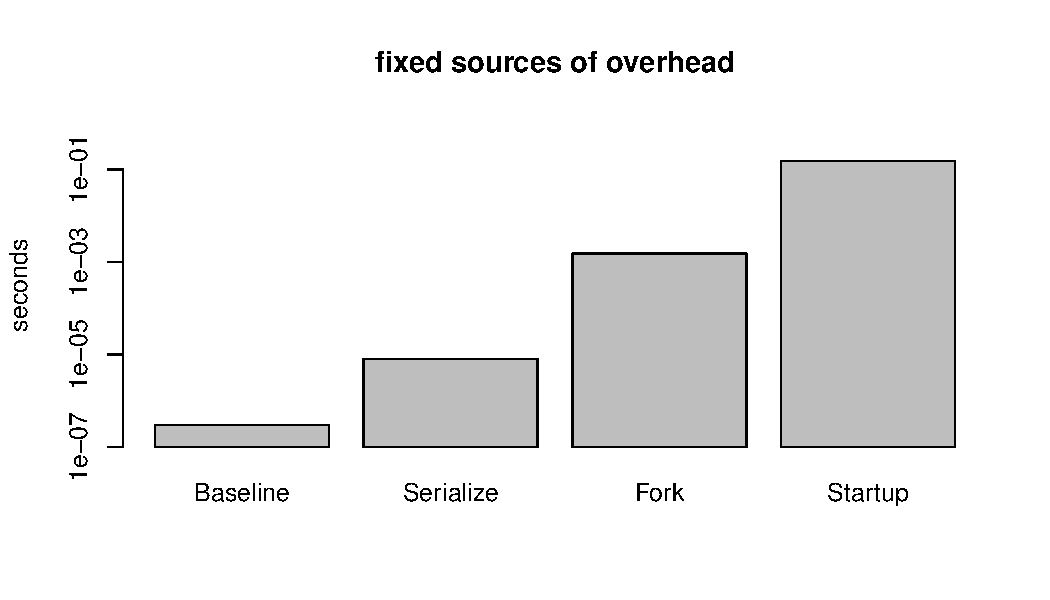
\includegraphics[width=.8\linewidth]{compute_times/overhead}

    \caption{
        This figure shows the overhead associated with various
    operations by measuring the time to execute with small data. 
    \emph{Baseline} calls \texttt{twox(10)} where \texttt{twox = function(x) 2*x}.
    \emph{Serialize} sends and receive an object on a local network socket connection.
    \emph{Fork} calls a system level fork of the process to evaluate a
    function, returning the result to the current process.
    \emph{Startup} starts a new independent instance of the R interpreter.
    }
\label{fig:overhead}
\end{figure}

% Maybe could take this out?
The evaluation of the following simple
function captures the basic overhead associated with an interpreted
language like R:
\begin{verbatim}
twox = function(x) 2*x
\end{verbatim}
Every call to this function will incur a fixed overhead that is a couple
hundred nanoseconds. Vectorization refers to passing longer vectors to the
function to amortize this fixed cost. For example, if $x$ is an integer
vector of length 1 then the overhead takes 2 orders of magnitude more time
than the actual computation. However, if $x$ is of length 1500 then this
overhead accounts for only 10 percent of the total execution time, so the
fixed cost has been amortized.

\subsection{Expression Dependency Graphs}

\label{sec:expression_dependency}

We build on the CodeDepends package \cite{R-CodeDepends} for static code
analysis.  The evaluation model for interpreted languages is simple. Each
expression of code is evaluated in the order that it appears in a text
file. Informally each expression is a line of code. This can be viewed as a
set of constraints on the evaluation order of the expressions:

\begin{itemize}
    \item expression 1 executes before expression 2
    \item expression 2 executes before expression 3
    \item $\dots$
\end{itemize}
What if these constraints are relaxed? Suppose expression 1 defines the variable
\texttt{x}, which is not used until expression 17. Then one has the
constraint:
\begin{itemize}
    \item expression 1 executes before expression 17
\end{itemize}
This can be generalized into a directed graph which we'll refer to here as
the \textbf{expression dependency graph} by considering expressions as
nodes and constraints as edges. The edges are implicit based on the order
of the statements in the code. There is an edge from $i \rightarrow k$ if
expression $k$ depends on the execution of expression $i$.  It's safe to
assume $i < k$, because expressions appearing later in a program can't
affect expressions which have already run. Hence the expression graph is
acyclic, i.e. a DAG. The expression graph differs from a control flow
graph because it treats control flow constructs such as \texttt{for()}
loops as top level expressions and functions, just like the R interpreter.
It would be possible to go into the control flow, but this can be done more
efficiently at the R compiler level.

Figure~\ref{fig:ast} and figure~\ref{fig:codegraph} illustrate the 
parse tree and expression dependency graph for the simple script on
page~\pageref{list:ab}.  Edges 1 and 3 in figure \ref{fig:codegraph} represent the
respective uses of the variable \texttt{n} and \texttt{x}.  Edge 2 comes
from the redefinition of \texttt{n}.  Edge 5 propagates the most recent
definition of \texttt{n}.  The least obvious is edge 4, which is necessary
to respect R's lexical scoping semantics since \texttt{x <- rnorm(n)} uses
the first definition of \texttt{n}. The general rule here is that all
statements using one version of the variable \texttt{n} must execute before \texttt{n}
can be redefined.

\lstinputlisting[language=R, caption=Simple script, label=list:ab]{../experiments/ast/ab.R}

\begin{figure}
\centering
\begin{subfigure}{.6\textwidth}
    \centering
    \includegraphics[width=.8\linewidth]{../experiments/ast/ast.pdf}
    \caption{Parse tree}
    \label{fig:ast}
\end{subfigure}%
\begin{subfigure}{.4\textwidth}
  \centering
  \includegraphics[width=.8\linewidth]{../experiments/ast/codegraph.pdf}
  \caption{Expression dependency graph}
  \label{fig:codegraph}
\end{subfigure}
\caption{Different representations of the script in Listing \ref{list:ab}}
%\label{fig:test}
\end{figure}

The expression dependency graph provides a tool for going beyond
embarrassingly parallel problems, since some subgraphs may potentially run
in parallel. In practice, I could not find real examples in R code where
the benefits of this type of parallelism outweigh the overhead, but with
threads it may be possible. This graph is still useful for understanding
the structure of the code.

\subsection{Entry points for parallelism}

\label{sec:parallel_points}

Three types of functions in R are of special interest when doing parallel
computation: apply functions, vectorized functions, and reduce functions.

Apply functions are higher order functions which call the same function
with potentially different arguments. Conceptually, they are variations to the ``map''
step in the map reduce paradigm \cite{dean2008mapreduce}.  In base R these
include \texttt{lapply, apply, sapply, vapply, Map, mapply, by, tapply,
outer, replicate}. These should be the first target for parallelism because
they are closest to the existing technologies, ie. \texttt{lapply()} has a
corresponding function \texttt{mclapply()} in the parallel package.

Vectorized functions apply functions elementwise. Basic math functions such
as sin, log, and floor are simple examples of vectorized functions.  A
vectorized function $f$ operating on an argument $x$ of length $n$ does:
\begin{equation}
\label{eq:vectorization}
    f(x) = (f(x_1), \dots, f(x_n))
\end{equation}
Partitioning $x$ into $p$ subvectors, 
\[
    x = \left[ (x_{11}, \dots, x_{1 n_1}), \dots, (x_{p 1}, \dots, x_{p
n_p}) \right]
\]
allows us to parallelize $f(x)$ by evaluating $f$ on the subvectors as follows:
\[
    f(x) = \left[ f(x_{11}, \dots, x_{1 n_1}), \dots, f(x_{p 1}, \dots, x_{p
n_p}) \right].
\]
If the subvectors are large enough then this can be efficient in R also.
However, the overhead of splitting $x$ into subvectors, evaluating in
parallel, and recombining $f(x)$ may take more time than calling $f()$
itself. It becomes more efficient when combined with a reduce function,
since there's less data to recombine.

The general form of the \texttt{Reduce()} function in R collapses elements
into a single result by calling a function $f()$ repeatedly on the
elements. For example \texttt{Reduce(`+`, 1:4)} is equivalent to
\texttt{(((1 + 2) + 3) + 4)}. Common examples that can be written this way
include \texttt{min, max, mean, sum, prod}. A more interesting example is
to simultaneously join many data frames through \texttt{Reduce(merge,
...)}.  Since we're computing on large data sets numerically stable
algorithms should be used here, ie.  Kahan summation \cite{Robey2011217}.
Reduce style functions can be used to reduce the size of the data in a
worker before transferring to the manager.

\subsection{Challenges}

It would be quite ambitious to produce a complete system capable of
producing optimal code on such different systems as multicore, GPU, and
distributed. Some of the foundational capabilities aren't yet mature, i.e.
compiling R code to an OpenCL kernel which runs on a GPU. Moreover, the
semantics across the systems may differ. For example, a file backed
\texttt{matrix} from the \texttt{bigmemory} package has reference
semantics, unlike an ordinary R matrix \cite{bigmemory}.

Non standard evaluation and dynamic scoping rules make some of the
static code analysis difficult. For example, to fit a linear model with
\texttt{lm(y\textasciitilde x, data)}, it's possibe that $x$ is a global variable while
$y$ is a column name in \texttt{data}. Generally this can't be known until
run time, since one could have the following code which randomly assigns
$x$:

\begin{verbatim}
x = 1:10
if(sample(c(TRUE, FALSE), 1)){
    data$x = rnorm(10)
}
\end{verbatim}

When identifying global variables to send to workers one can do the
conservative thing and send both \texttt{x, data}.

Another challenge is handling mutable or more complex objects
such as environments, closures, and reference classes.  It's usually not
possible to know the class of an object until runtime. But user and package
code could be inspected to see if certain objects are used, for example by
looking for calls to the function \texttt{setRefClass()}. The code
analysis will have to respect the implicit connections between these
objects.

\section{Conclusion}
%%%%%%%%%%%%%%%%%%%%%%%%%%%%%%%%%%%%%%%%%%%%%%%%%%%%%%%%%%%%

\subsection{Interfaces}

Parallel programming in pure R (not at the C level) can be understood in
terms of a layered architecture. The foundational \textbf{System Layer}
provides the basic interfaces used by any programming language. The
\textbf{R Layer} consists of packages which adapt the basic interfaces for
use specifically in R. The packages in the \textbf{User Layer} are meant to
simplify parallel programming, or they are for applications with specific
use cases.  Here are a few examples of packages at each layer:

\begin{itemize}
\item User Layer: foreach, future, partools, ddR, biganalytics, RevoScaleR
\item R layer: SNOW, multicore, parallel, bigmemory, Rmpi
\item System Layer: processes, *NIX fork(), memory maps, network sockets,
    MPI
\end{itemize}

Today users write code using packages from the User Layer or the R Layer.
Modifying code programmatically can allow us to skip these layers, and
instead write the same base R code which will run in serial as in parallel.
This is appealing for two reasons. Base R is stable, so users can write
code that works locally as in parallel, and can expect it to continue to
work in the future. Second, if the code runs on a different system or with
a different data set then one can automatically generate code to run more
efficiently on that system.

Some of the work in this project may mean enhancing the capabilities of these
intermediate layers. For example, a file based sort usable from R facilitiates
``group by'' and streaming applications.

\subsection{Related Technologies}

Related technologies include Theano, tensorflow, dask, and arrayfire. With
these packages the user explicitly builds computation graphs which are then
executed in an efficient way based on the available architecture. They are
more tailored to linear algebra / numerical computing, and are particularly
popular for implementing neural networks. One possible path to explore is
the translation of R code into these systems. This might be difficult when
processing non numeric data.

\subsection{Next Steps}

My immediate plan is to build the infrastructure to analyze the highway
sensor data within this more general framework. I plan to see the analysis
through to a stage where it can be shared with the transportation research
community.  At a minimum this means preprocessing tools, profiling tools,
and a parallel group by. The target \emph{platform} is a single server, and
the \emph{data} consists of files which may exceed memory.

After this I plan to find another use case for parallel processing of data
in a different format, either in a database or in a streaming system such
as Apache Kafka.

\bibliographystyle{plain}
\bibliography{../citations,../Rpackages} 

\end{document}
